\documentclass[10pt]{article}
\usepackage[utf8]{inputenc}
\usepackage[english]{babel}
\usepackage[font=small,labelfont=bf]{caption}
\usepackage{geometry}
\usepackage[sort&compress, numbers, super]{natbib}
\usepackage{pxfonts}
\usepackage{graphicx}
\usepackage{setspace}
\usepackage{hyperref}
\usepackage{lineno}

\newcommand{\argmax}{\mathop{\mathrm{argmax}}\limits}

%\newcommand{\demo}{S1}

\doublespacing
\linenumbers

\title{Carryover effects in free recall reveal how prior experiences influence memory for new experiences}
\author{Jeremy R. Manning\textsuperscript{1, *}, Andrew C. Heusser\textsuperscript{1, 2}, Kirsten Ziman\textsuperscript{1, 3},\\Emily Whitaker\textsuperscript{1}, and Paxton C. Fitzpatrick\textsuperscript{1}\\\textsuperscript{1}Dartmouth College\\\textsuperscript{2}Akili Interactive\\\textsuperscript{3}Princeton University\\\textsuperscript{*}Corresponding author: jeremy.r.manning@dartmouth.edu}

\date{}

\begin{document}
\maketitle

\begin{abstract}
We perceive, interpet, and remember ongoing experiences through the lens of our prior experiences.
Inferring that we are one type of situation versus another can lead us to interpret the same physical
experience differently.  In turn, this can affect how we focus our attention, form expectations of what will happen next, 
remember what is happening now, draw on our prior related experiences, and so on.  To study these phenomena,
we asked participants to perform simple word list learning tasks.  Across different experimental conditions, we held the set of
to-be-learned words constant, but we manipulated the orders in which the words were studied.  We found that 
these order manipulations affected not only how the participants recalled the ordered lists, but also how they recalled later randomly
ordered lists.  Our work shows how structure in our ongoing experiences can exert influence on how we remember unrelated
subsequent experiences.
\end{abstract}


\section*{Introduction}

% the role of context and prior experience in memory

% situation models: forming expectations, predicting ambiguous future experiences

% gap between "classic" free recall tasks and naturalistic (or real-world) memory tasks

% feature-rich free recall, basic manipulation conditions, preview of findings

\section*{Results}

\begin{figure}[tp]
    \centering
    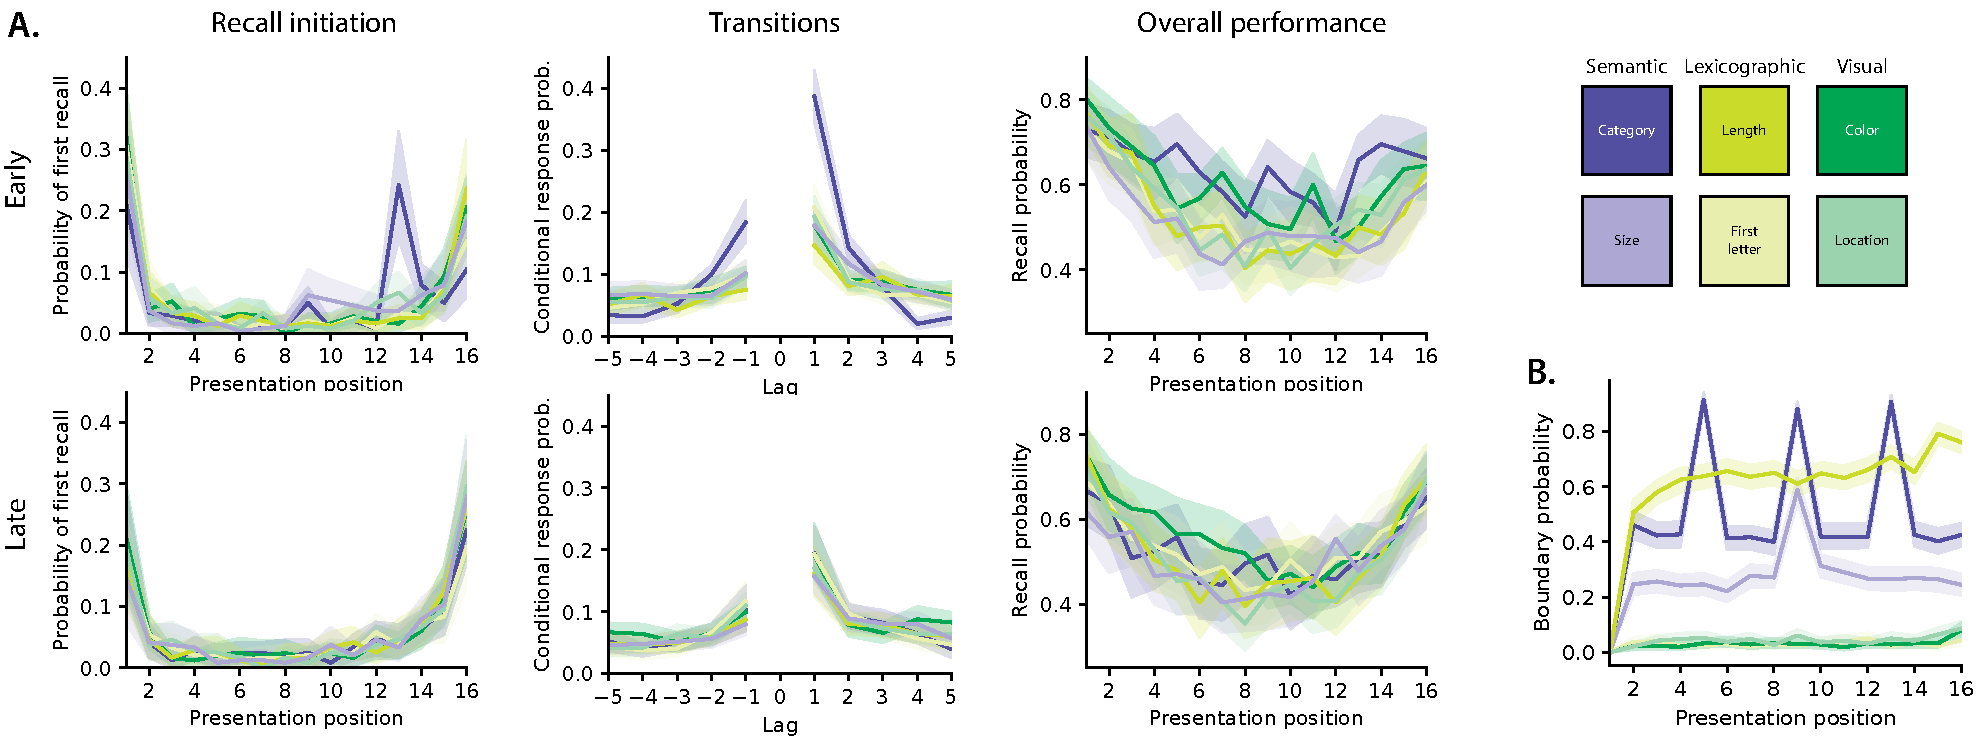
\includegraphics[width=\textwidth]{figures/recall_dynamics}
    \caption{\textbf{Recall dynamics in free recall.}}
    \label{fig:recall-dynamics}
\end{figure}

% figure: clustering effects

% figure: recall initiation

% figure: feature clustering vs. accuracy, feature clustering vs. temporal clustering

% figure: fingerprint trajectories

% figure: carryover effects: clustering early vs. clustering late

% figure: clustering carryover vs. accuracy difference

% figure: clustering carryover vs. temporal clustering differences

\section*{Discussion}

% recap

% connections to prior work: context effects, priming, situation models

% implications for adaptive learning, education and training


\section*{Materials and methods}
\subsection*{Participants}

\subsection*{Experimental design}

\subsection*{Analysis}

\bibliographystyle{apa}
\bibliography{cdl}
\end{document}
